\chapter{Requirements Engineering}
Quando si parla di \textbf{requirements engineering} (RE) di fatto ci si concentra
sulla comprensione di come una soluzione software si deve comportare per risolvere
un certo problema. In questo senso bisogna prima comprendere quale sia il problema
da risolvere e in quale contesto tale problema si verifica, per poter arrivare
ad una soluzione corretta ed efficacie a problemi reali. Bisogna ben comprendere
il problema, non si parla quindi della progettazione in se, ma del “cosa” deve
fare il software.

Vediamo ora l'analogia classica per spiegare il RE, il problema mondo e la soluzione
macchina. Si hanno:
\begin{itemize}
    \item Il \textbf{mondo}, con un problema derivante dal mondo reale, mondo
          stesso che produce tale problema che bisognerà risolvere con un calcolatore.
    \item La \textbf{macchina}, che bisogna sviluppare per risolvere il problema.
    \item \textbf{Requirements engineering} che si occupa di definire gli effetti
          della macchina sul problema del mondo e definire assunzioni e proprietà
          principali del mondo stesso.
\end{itemize}

Macchina e mondo possono condividere alcuni componenti, con la macchina che
modifica il mondo. Nel requirements engineering studiamo quindi il mondo, senza
definire come funziona internamente la macchina.

Quando si parla di requirements engineering è bene distinguere due elementi:
\begin{itemize}
    \item Ogni volta che prendiamo in considerazione un problema esiste sempre
          un \textbf{system-as-is}, ovvero un sistema preesistente che già risolve il
          problema. Si ha quindi sempre un sistema da cui partire.
    \item Esiste sempre un \textbf{system-to-be}, ovvero il sistema che si andrà
          a realizzare. In altre parole è il sistema quando la macchina/software ci
          opera sopra.
\end{itemize}

Studiare il system-as-is è essenziale per poter lavorare al system-to-be.
\begin{definizione}[\textbf{requirements engineering}]
    Il \textbf{requirements engineering} è, formalmente, un insieme di attività:
    \begin{itemize}
        \item Per esplorare, valutare, documentare, consolidare, rivisitare e
              adattare gli obiettivi, le capacità, le qualità, i vincoli e le ipotesi
              su un system-to-be.
        \item Basate sul problema sorto dal system-as-is e sulle nuove opportunità
              tecnologiche.
    \end{itemize}
    L'output di queste attività è un documento di specifica dei requisiti con
    tutto ciò che soddisfa il sistema. Se l'output non è un singolo documento si
    ha una collezione di singoli requisiti, che nel metodo agile sono storie/cards
    e in altri metodi un repository centrale con un db condiviso contenete i
    vari requisiti.

    In ogni caso si ha un insieme di requisiti su come si deve comportare il
    sistema che si andrà a realizzare.
\end{definizione}

In un modello di sviluppo a cascata requirements engineering è una delle primissime
attività, subito dopo quelle di definizione del sistema e di business plan.

Per gli aspetti tecnici è probabilmente la prima attività svolta, occupandosi di
ottenere il giusto sistema da sviluppare, prima di design, implementazione ed
evoluzione software etc$\dots$ che si occupano di ottenere il software giusto,
sviluppandolo nel modo corretto.

Errare nel requirements engineering può portare ad un ottimo software che risolve
i problemi sbagliati oppure a un software che non risolve tutti i problemi che
dovrebbe risolvere. Sbagliare il requirements engineering è una causa di
fallimento del progetto.

Lavorare sui requirements non è semplice per diversi motivi:
\begin{itemize}
    \item Si deve ragionare su tante versioni del sistema come il system as-is,
          il system to-be e il system to-be-next, volendo essere lungimiranti per il
          comportamento del sistema, sapendo e prevedendo evoluzioni future.
    \item Si lavora in ambienti ibridi in un contesto che va compreso a fondo.
    \item Si hanno diversi aspetti funzionali, qualitativi e di sviluppo.
    \item Si hanno diversi livelli di astrazione, con obiettivi strategici a
          lungo termine di inserimento sul mercato e dettagli operazionali.
    \item Si hanno tanti stakeholders, quindi con diverse parti interessati di
          cui risolvere problemi e interessi con potenziali conflitti tra i vari
          stakeholders.
    \item Si hanno tante attività tecniche legate l'una con l'altra:
          \begin{itemize}
              \item Conflict management
              \item Risk management
              \item Evaluation of alternatives
              \item Prioritization
              \item Quality assurance
              \item Change anticipation
          \end{itemize}
\end{itemize}
\section{Tipi di requisiti}
Bisogna anche ragionare sui tipi di requisiti su cui si deve lavorare. Una prima
differenza si ha nel modo in cui sono scritti i requisiti. Si hanno quindi:
\begin{itemize}
    \item \textbf{Descriptive statements}: indicano dei requisiti non negoziabili,
          rappresentano dei comportamenti derivanti dalle leggi del mondo su cui
          lavora. Si ha quindi zero margine di modifica.
    \item \textbf{Prescriptive statements}: indicano requisiti negoziabili.
\end{itemize}

Entrambi sono importanti e vanno considerati. Si possono avere requisiti non ovvi,
o lo sono in un contesto specialistico e quindi spesso non ovvi a chi lavora
sul software, che magari nemmeno sa che esistono.

I requisiti possono inoltre differire per gli elementi che prendono in considerazione.
Posso avere requisti:
\begin{itemize}
    \item \textbf{System requirements}: come si comporta l'ambiente, per capirne
          il funzionamento.
    \item \textbf{Software requirements}: come si comporta il software
          nell'ambiente, studiando i cosiddetti shared fenomena.
\end{itemize}
ricordando che:
\begin{center}
    Sistema = Ambiente + Software \\ System requirements = Software requirements
    + Domain Properties + Assumption
\end{center}
I requisti comunque non riguardano mai il comportamento interno del software.
\newline Si hanno 3 dimensioni:
\begin{enumerate}
    \item \textbf{Dimensione del why}: si identificano, analizzano e rifiniscono
          i requisiti del system-to-be per affrontare le carenze analizzate del
          system-as-is, in linea con gli obiettivi di business, sfruttando le opportunità
          tecnologiche. Si hanno le seguenti difficoltà:
          \begin{itemize}
              \item Acquisire conoscenza del dominio
              \item Valutare opzioni alternative
              \item Abbinare problemi-opportunità e valutarli in termini di implicazioni,
                    e rischi associati.
              \item Gestire obiettivi contrastanti.
          \end{itemize}
    \item \textbf{Dimensione del what}: si identificano, analizzano e rifiniscono
          le funzionalità del system-to-be per soddisfare gli obiettivi individuati in
          base a vincoli basati su ipotesi realistiche sull'ambiente. Si hanno le seguenti difficoltà:
          \begin{itemize}
              \item Identificare il giusto set di funzionalità.
              \item Specificarle precisamente per essere comprese da tutte le parti.
              \item Garantire la tracciabilità backward per gli obiettivi del sistema.
          \end{itemize}
    \item \textbf{Dimensione del who}: si assegna responsabilità per gli obiettivi,
          i servizi, i vincoli tra i componenti del system-to-be in base alle loro
          capacità e agli obiettivi del sistema, oltre i confini dell'ambiente software.
          La difficoltà è valutare opzioni alternative per decidere il giusto grado
          di automazione.
\end{enumerate}

I requisti che riguardano l'ambiente possono essere di due forme:
\begin{itemize}
    \item \textbf{Domain properties}: proprietà riguardanti l'ambiente, immutabili.
    \item \textbf{assumptions}: su come è fatto l'ambiente. Il software funzionerà
          solo negli ambienti che soddisfano quella certa assunzione. Se troppo
          restrittive possono portare al fallimento del progetto, che riguarderebbe
          pochissimi casi particolari.
\end{itemize}
\begin{definizione}[\textbf{Domain property}]
    Definiamo \textbf{domain property} come un descriptive statement sui problemi
    legati ai fenomeni del mondo (a prescindere da qualsiasi software-to-be).
    $\text{Domain property} \  \subseteq M \times C$ se leggi che non possono
    essere infrante.
\end{definizione}
Si ha che:
\begin{center}
    Software requirements = \textit{map}(System requirements, Software requirements,
    Domain property)
\end{center}

È utile quindi fare una distinzione per quanto concerne i requisiti del software.
Abbiamo due famiglie principali:
\begin{itemize}
    \item \textbf{Requisiti funzionali}, che indicano le funzionalità che un
          sistema (system-to-be) deve implementare, cosa deve essere in grado di fare.
          Non sono prevedibili prima di studiare il sistema.
    \item \textbf{Requisiti non funzionali}, che indicano delle qualità o dei
          vincoli sulle funzionalità e quindi sui requisiti funzionali. Questa famiglia
          di aspetti non funzionali è più o meno standard.
\end{itemize}

Per l'identificazione dei requisiti non funzionali si può utilizzare una
\textit{tassonomia}, riportata in figura \ref{fig:tasso}, dove si trovano organizzati
aspetti non funzionali tali per cui, dopo aver individuato le funzionalità posso
ricercare eventuali requisiti non funzionali.
\begin{figure}[!ht]
    \centering
    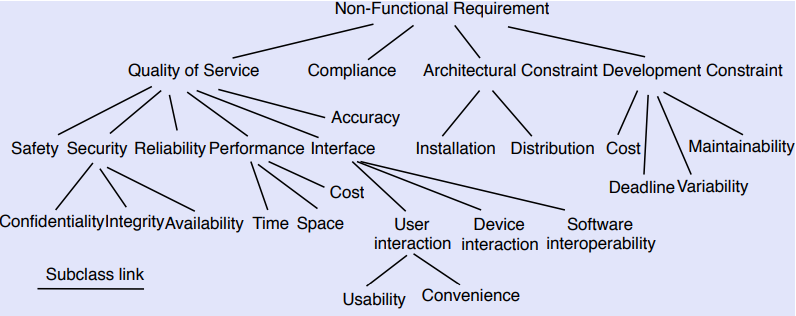
\includegraphics[width=0.5\textwidth]{img/requirements/tassonomia.png}
    \caption{Tassonomia dei requisiti non funzionali}
    \label{fig:tasso}
\end{figure}
Per alcuni tipi di progetti requisiti funzionali e non funzionali sono difficilmente
distinguibili, spesso mischiandosi.
\section{Qualità dei requisiti}
Si hanno diversi aspetti di cui preoccuparsi nell'analisi dei requisiti. Si hanno
tante qualità indispensabili:
\begin{itemize}
    \item \textbf{Completezza}: è necessario descrivere tutti i requisiti rilevanti
          del progetto, identificando tutti i comportamenti del sistema e documentarli
          in modo adeguato. È una qualità virtualmente irraggiungibile in modo assoluto,
          non è infatti verificabile. Inoltre i requisiti variano al proseguire del
          progetto, interagendo anche con gli stakeholders, rendendo questo uno degli
          aspetti più difficili da studiare.
    \item \textbf{Consistenza}: i requisiti non devono presentare dei conflitti,
          dato l'elevato numero di requisiti è facile introdurre inconsistenze.
    \item \textbf{Non ambiguità}: tutto deve essere chiaro e non soggetto ad
          interpretazione.
    \item \textbf{Misurabilità}: non basato su interpretazioni vaghe ma si misure
          concrete e specifiche.
    \item \textbf{Fattibilità}: non si devono avere requisiti basati su
          funzionalità irrealizzabili.
    \item \textbf{Comprensibilità}.
    \item \textbf{Buona struttura}.
    \item \textbf{Modificabilità}: possibilità di avere il risultato mantenibile
          del tempo.
    \item \textbf{Tracciabilità}: individuando tutti gli artefatti ottenibili
          come conseguenza e tracciandoli. Si tracciano anche le dipendenze tra requisiti.
\end{itemize}
Vediamo quindi gli errori che si fanno quando si va ad identificare i requisiti:
\begin{itemize}
    \item \textbf{Omissioni}: non si riesce ad identificare qualche requisito.
          Anche un riconoscimento tardivo è un problema in quanto comporta la modifica
          del documento, non sempre facile.
    \item \textbf{Contraddizioni}: si presentano conflitti tra i requisiti.
    \item \textbf{Inadeguatezza}: requisiti che non sono adeguati per un determinato
          problema.
    \item \textbf{Ambiguità}: requisiti interpretabili.
    \item \textbf{Non misurabilità}: non si riesce a fornire una misura di certi
          requisiti, specialmente non funzionali, che comportano difficoltà di gestione,
          precludendo confronti etc$\dots$
\end{itemize}
Si hanno anche altri tipi di errore:
\begin{itemize}
    \item Essere troppo specifici nella definizione dei requisiti includendo
          anche comportamenti interni al software che non dovrebbero essere descritti
          in questa fase.
    \item Descrivere requisiti non implementabili considerando vincoli temporali
          o di costo.
    \item Descrivere requisti complessi da leggere.
    \item Avere poca struttura nella stesura dei requisiti, a livello visivo.
    \item Se si produce un documento bisogna evitare di fare riferimento a
          requisiti che non sono stati ancora descritti, ovvero evitando il forward
          reference.
    \item Evitare “rimorsi” di non aver definito nel momento giusto certi concetti
          che magari erano stati usati, senza definizione, precedentemente.
    \item Evitare la poco modificabilità del documento. È buona norma avere delle
          “costanti simboliche”, definite all'inizio, a cui fare riferimento nel documento,
          in modo che un'eventuale modifica si rifletta su tutto il documento.
    \item Evitare l'opacità/logica di fondo/rationale/motivazioni dei requisti,
          in modo che sia chiaro il perché esso è stato incluso, portando a mettere in
          discussione requisiti in realtà sensati a cui si arriverebbe comunque dopo
          ulteriore analisi, dopo aver perso ulteriore tempo.
\end{itemize}
\section{Il processo requirements engineering}
Si hanno 4 fasi a spirale (figura \ref{fig:spirale}):
\begin{figure}[!ht]
    \centering
    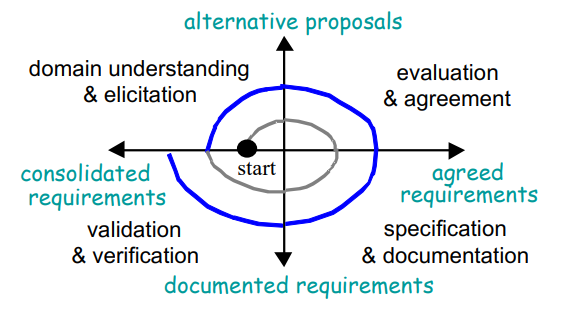
\includegraphics[width=0.6\textwidth]{img/requirements/spirale.png}
    \caption{Rappresentazione modello a spirale}
    \label{fig:spirale}
\end{figure}
\begin{enumerate}
    \item \textbf{Domain understanding} $\&$ \textbf{elicitation}: in questa fase
          si hanno due parti principali:
          \begin{itemize}
              \item \textbf{Domain understanding}: in questa fase si ha  lo studio del
                    system-as-is in ottica di studio del dominio applicativo, studio del business
                    organizzazione che vuole il prodotto. Si studiano anche forze e debolezze del
                    system-as-is. Si studia il dominio applicativo per ottenere il miglior
                    system-to-be possibile. Inoltre, si identificano gli stakeholders del
                    progetto per poter capire a fondo interessi e fini.

                    Come output di questa fase si hanno le sezioni iniziali per la bozza di
                    proposta preliminare e il glossario dei termini.
              \item \textbf{Requirements elicitation}: studio più approfondito nel mondo
                    attraverso un'ulteriore analisi dei problemi legati al system-as-is.
                    Inoltre, vengono identificati, grazie all'aiuto degli stakeholders:
                    \begin{itemize}
                        \item Opportunità tecnologiche.
                        \item Condizioni del mercato
                        \item Obiettivi di miglioramento
                        \item Vincoli, organizzativi e tecnici, del system-as-is
                        \item Alternative per raggiungere l'obiettivo e assegnare le responsabilità.
                        \item Scenari di ipotetica interazione software-ambiente
                        \item Requisiti del software
                        \item Assunzioni sull'ambiente
                    \end{itemize}
                    In in output si hanno ulteriori sezioni per la bozza di proposta preliminare.
          \end{itemize}
    \item \textbf{Evaluation} $\&$ \textbf{agreement}: si effettuano decisioni
          basate sull'interazione con i vari stakeholders, per poter valutare e decidere,
          avendo cambiamenti dei rischi in base a:
          \begin{itemize}
              \item Identificazione e risoluzione di conflitti di interesse.
              \item Identificazione e risoluzione di rischi legati al sistema proposto.
              \item Comparazione e scelta tra le alternative proposte in merito a
                    obiettivi e rischi.
              \item Prioritizzazione dei requisti, al fine di risolvere conflitti,
                    definire vincoli di costi e tempi, supportare lo sviluppo incrementale.
          \end{itemize}
          In in output a questa fase si hanno le sezioni finali per la bozza di proposta
          preliminare, dove si documentano gli obiettivi selezionati, i requisiti, le
          assunzioni e il rationale, la logica di fondo delle opzioni selezionate.
    \item \textbf{Specification} $\&$ \textbf{documentation}: in questa fase si
          raccoglie quanto detto nelle prime due fasi per produrre il documento, si hanno quindi:
          \begin{itemize}
              \item Definizione precisa di tutte le funzionalità del sistema scelto,
                    tra cui:
                    \begin{itemize}
                        \item Obiettivi, concetti, proprietà rilevanti del dominio d'interesse,
                              requisti del sistema, requisti del software, assunzioni sull'ambiente
                              e responsabilità.
                        \item Motivazioni e logica di fondo delle opzioni scelte.
                        \item Probabili evoluzioni del sistema ed eventuali variazioni.
                    \end{itemize}
              \item Organizzazione di quanto appena citato in una struttura coerente
              \item Documentazione del tutto in un formato comprensibile a tutte le parti,
                    mettendo in allegato:
                    \begin{itemize}
                        \item Costi
                        \item Piano di lavoro
                        \item Tempi di consegna del risultato
                    \end{itemize}
          \end{itemize}
          In output a questa fase si ha il vero e proprio \textbf{Requirements Document}
          (RD).
    \item \textbf{Validation} $\&$ \textbf{verification}: in questa fase si studia
          il requirements document, ovvero si studia la garanzia di qualità del
          requirements document, analizzando varie attività:
          \begin{itemize}
              \item Validazione, ovvero vedendo se quanto contenuto nel requirements
                    document è adeguato con quanto si necessita
              \item Verifica, controllando se ci sono omissioni o inconsistenze
              \item Correzione di eventuali errori e difetti
          \end{itemize}
          In output a questa fase si ha un requirements document consolidato.
\end{enumerate}

Come è stato detto queste quattro fasi si ripetono in modo iterativo in modo “a
spirale”. Questo viene fatto in quanto si possono avere evoluzioni nel processo
nonché correzioni di quanto già fatto che si propagano su tutto il documento. Le
evoluzioni e le correzioni possono sopraggiungere durante:
\begin{itemize}
    \item Il requirements engineering stesso.
    \item Lo sviluppo del software.
    \item Dopo il deploy del software stesso.
\end{itemize}
Dopo ogni ciclo si è molto più consci del sistema e si può passare al miglioramento
del requirements engineering con più efficacia.
\subsection{Domain understanding \& elicitation}
Iniziamo analizzando la fase di \textbf{elicitation}, la quale consiste in un
insieme di tecniche atte allo scoprire requisiti che un progetto deve soddisfare.
\subsubsection{Stakeholders}
La selezione degli stakeholders del progetto è la prima fase che viene svolta
per poter lavorare alla elicitation.
\begin{definizione}[\textbf{Stakeholder}]
    In generale uno \textbf{stakeholder} è un'organizzazione o una persona che
    nutre un interesse rispetto al progetto. Si hanno diversi aspetti per la
    selezione degli stessi:
    \begin{itemize}
        \item Posizione nell'organizzazione.
        \item Ruolo nel prendere decisioni sul system-to-be.
        \item Livello di esperienza del dominio applicativo.
        \item Esposizione al problema che il sistema deve risolvere.
        \item Influenza nell'accettazione del sistema.
        \item Obiettivi personali ed eventuali conflitti di interesse.
    \end{itemize}
\end{definizione}
Conoscendo gli stakeholders avremo modo di prendere in considerazioni gli interessi
degli stakeholders tramite diverse strategie. Idealmente si vuole realizzare
qualcosa che soddisfi gli interessi di tutti gli stakeholders.

Questa è un'attività insidiosa in quanto non si può dire se l'insieme degli
stakeholders sia completo. Si hanno anche stakeholders non sono dell'organizzazione
ma anche associazioni, ulteriori organizzazioni, addetti alle normative di settore
e così via. Si hanno anche stakeholders che non interagiscono direttamente col sistema.

Un modo per identificare gli stakeholders è tramite una serie di semplici domande,
tramite una piccola attività di brainstorming:
\begin{itemize}
    \item Chi è influenzato positivamente e negativamente dal progetto?
    \item Chi ha il potere di fargli avere successo (o farlo fallire)?
    \item Chi prende le decisioni in materia di denaro?
    \item Chi sono i fornitori?
    \item Chi sono gli utenti finali?
    \item Chi ha influenza, anche indiretta, sugli altri stakeholder?
    \item Chi potrebbe risolvere potenziali problemi con il progetto?
    \item Chi si occupa di assegnare o procurare risorse o strutture?
    \item Chi ha competenze specialistiche cruciali per il progetto?
\end{itemize}
Dimenticare uno stakeholders può portare ritardi o fallimenti del progetto, dovendo
rivedere magari requisti o dovendo rifare parti di sviluppo. Si hanno varie
difficoltà nell'acquisire informazioni dagli stakeholders, rendendo complesso il dialogo:
\begin{itemize}
    \item Fonti di conoscenza sul sistema distribuite sui vari stakeholders e tali
          fonti spesso sono contrastanti.
    \item Accesso difficile alle fonti
    \item Ostacoli alla buona comunicazione, avendo background diversi sul dominio.
    \item Conoscenza non comunicata esplicitamente e bisogni nascosti
    \item Fattori socio-politici
    \item Condizioni instabili e mutabili, cambiano gli stakeholders, si hanno
          dinamiche aziendale mutevoli e cambi di ruoli. Anche per questo si hanno i metodi agili.
\end{itemize}

Servono quindi buone capacità comunicative, sapendo usare la giusta terminologia
di dominio, arrivando dritti al punto e creando un rapporto di fiducia con gli
stakeholders. Si ha inoltre un piccola pratica, detta knowledge reformulation,
ovvero quando si acquisiscono informazioni anche da fonti multiple è bene riformulare
tale informazione allo stakeholder, per verificare una corretta comprensione.

È bene fare distinzione sulle tecniche di engagement con gli stakeholders,
considerando due variabili, catalogandole in low e high:
\begin{enumerate}
    \item \textbf{Potere decisionale}.
    \item \textbf{Interesse nel progetto}.
\end{enumerate}
Si ha quindi una classificazione degli stakehlders in base a queste due variabili:
\begin{table}[!ht]
    \centering
    \begin{tabular}{c|c|c}
        \textbf{Potere} & \textbf{Interesse} & \textbf{Strategia} \\\hline
        high            & high               & Fully engage       \\
        high            & low                & Keep satisfied     \\
        low             & high               & Keep satisfied     \\
        low             & low                & Minimum effort
    \end{tabular}
\end{table}
Dove nel dettaglio:
\begin{itemize}
    \item \textbf{Fully engage}: implica un coinvolgimento regolare degli
          stakeholders che in questo caso sono della categoria principale.
    \item \textbf{Keep satisfied}: si hanno due casi:
          \begin{itemize}
              \item Se hanno alto potere decisionale si cerca di mantenerli informati
                    e soddisfatti ma senza troppi dettagli.
              \item Se hanno alto interesse, essendo spesso gli end-user, si cerca di
                    consultarli spesso cercando di risolvere le problematiche indicate, coinvolgendoli
                    regolarmente per ottenere dettagli e informazioni specifiche, essendo
                    spesso i più informati sui dettagli.
          \end{itemize}
    \item \textbf{Minimum effort}: mentendoli informati in modo generale e
          monitorandone eventuali cambi di ruolo, potere o interesse.
\end{itemize}
\subsubsection{Elicitation techniques}
Passiamo quindi alle tecniche di elicitation. Si hanno due famiglie principali:
\begin{itemize}
    \item \textbf{Artefact-driven}: uso di artefatti per poter scoprire requisiti.
          \begin{enumerate}
              \item \textbf{Background study}, ovvero collezionare leggere e sintetizzare
                    documenti su:
                    \begin{itemize}
                        \item le organizzazioni stesse, ovvero grafici, business plan, report
                              finanziari, tempi delle riunioni $\dots$
                        \item il dominio applicativo, ovvero libri, paper, report su sistemi
                              simili $\dots$
                        \item il system-as-is, ovvero workflow documentati, procedure, regole
                              di business, report di errori, richieste di cambiamenti $\dots$
                    \end{itemize}
                    Queste collezioni di dati ci permettono di informarci in modo autonomo
                    sul mondo in cui si andrà a lavorare, senza coinvolgere lo stakeholders,
                    in quanto costoso, dispendioso e limitato in termini di tempo. Gli
                    stakeholders vanno interpellati non per informazioni reperibili autonomamente
                    ma per estrarre conoscenza non pubblica e non documentata. Ci si presenta
                    allo stakeholder già con una base di conoscenza e conoscendo già la
                    terminologia corretta del dominio.

                    Si ha quindi l'attività di data collection dove si estraggono informazioni
                    utili per studiare il target. Si possono fare attività di survey. Si
                    collezionano dati anche già documentati.

                    L'attività di background study ha ovviamente dei limiti di scalabilità,
                    non potendo leggere troppe cose, sia per tempo che per costo. Si ha quindi
                    la meta-knowledge per selezionare le parti dei documenti più rilevanti.
                    Queste attività sono essenziali all'avvio di un progetto.
              \item \textbf{Questionari}, ovvero una lista di questioni da presentare
                    agli stakeholders con una lista di possibili risposte. Si possono così
                    interrogare molti stakeholders contemporaneamente, senza una particolare
                    selezione. Si hanno quindi domande spesso a risposta multipla e raramente
                    aperte. Le domande devono essere chiare e che portino a risposte
                    affidabili. È bene fare pochi questionari efficaci, con risposte poco
                    affette da rumore. Si deve avere una numerosità di domande adeguata.
                    Questi questionari aiutano a preparare colloqui/interviste mirati più
                    efficaci. Spesso si usa prima un piccolo campione per i questionari per
                    poi mandarlo a tutti. Si devono evitare ambiguità e inserimenti di
                    bias, ne positivo ne negativo, nelle domande, senza avere domande che
                    possano condizionare la risposta. La raggiungibilità dei soggetti scelti
                    è essenziale, nonché la scelta degli stessi. È buona pratica avere domande
                    di cross-check per controllare chi sta rispondendo non dia risposte
                    inconsistenti e incoerenti, sintomo del fatto che uno non risponda a
                    caso.
              \item \textbf{Storyboards}: narrazioni, tramite esempi, di uso del sistema,
                    sia del system-as-is che del system-to-be. Sono quindi storie fatte tramite
                    sequenze di snapshots. Tali storie si creano in due modi:
                    \begin{itemize}
                        \item \textbf{Attivo}, dove lo stakeholder contribuisce alla costruzione
                              della narrazione.
                        \item \textbf{Passivo}, dove si narra la storia costruita allo
                              stakeholder.
                    \end{itemize}
                    Ovviamente vengono fatte solo per i workflow chiare.
              \item \textbf{Scenari} che descrivono, attraverso una sequenza di interazioni
                    rappresentate con testi o diagrammi, l'utilizzo del sistema, sia as-is che
                    to-be. L'uso di esempi rende semplice la comunicazione e l'interazione con
                    gli altri. Si hanno 4 tipi di scenario:
                    \begin{itemize}
                        \item \textbf{Positivo}, ovvero come il sistema si dovrebbe comportare
                        \item \textbf{Negativo}, ovvero cosa il sistema non dovrebbe fare
                        \item \textbf{Normale}, ovvero tutto procede come dovrebbe
                        \item \textbf{Anormale}, ovvero cosa succede in casi eccezionali
                    \end{itemize}
                    Gli ultimi due sono sotto-categorie degli scenari positivi.

                    Gli scenari sono un metodo naturale di interazione con lo stakeholders e
                    possono guidare la stesura di testi di accettazione. Hanno comunque dei
                    limiti, essendo solo esempi parziali e sono poco adatti alla combinazione
                    tra essi. Gli esempi possono anche deviare la comprensione del sistema,
                    che magari può comportarsi in molti altri modi, avendo anche dettagli
                    irrilevanti.

                    Gli scenari non si prestano all'interazione con molti stakeholder, a
                    causa della variabilità di questi in ottica di conoscenza e posizione.
              \item \textbf{Prototipi} e \textbf{mock-up}: sono realizzati quando
                    l'obiettivo è quello di controllare l'adeguatezza di un requisito, che
                    viene mostrato in modo visuale nella sua ipotetica formula finale. Si
                    hanno quindi piccoli esempi del software in azione, chiarendo e verificando
                    che sia quello di cui l'utente ha bisogno. Ovviamente un mock-up non ha
                    la logica applicative ma risposte costruite a priori. A seconda del tipo
                    di mock-up il focus è su:
                    \begin{itemize}
                        \item funzionalità, se sono state comprese correttamente e in modo
                              esaustivo
                        \item UI e UX, avendo focus più orientati all'usabilità
                    \end{itemize}
                    Si parla di mock-up se dopo l'uso viene buttato e di prototipo se, in caso
                    di approvazione, viene usato come base del software o comunque riutilizzato
                    in qualche modo, fornendo eventualmente una base evolutiva del software finale.

                    Come pro si ha una sensazione di concretezza per lo stakeholder, anche
                    visuale, permettendo anche già una sorta di training sul software che si
                    produce. Spesso i mock-up sono costosi, inoltre la loro natura simulata
                    può produrre aspettative troppo alte, magari anche solo in termini di
                    prestazioni. In un'ottica di riuso un mock-up è spesso inutilizzabile a
                    causa del quick-and-dirty code. Si ha anche il knowledge reuse, per velocizzare
                    l'elicitation, riusando conoscenze pregresse da sistemi simili a quello
                    sotto studio. Si hanno 3 fasi:
                    \begin{enumerate}
                        \item Trarre conoscenze e informazioni rilevanti da altri sistemi
                        \item Trasporle nel sistema in studio
                        \item Convalidare il risultato, adattarlo se necessario e integrarlo
                              con la conoscenza del sistema già acquisita
                    \end{enumerate}
                    Tali conoscenze possono essere dipendenti o indipendenti dal dominio.
                    Si hanno i seguenti pro:
                    \begin{itemize}
                        \item analisti esperti riutilizzano naturalmente dall'esperienza
                              passata
                        \item riduzione degli sforzi di eliciation
                        \item ereditarietà della struttura e qualità delle specifiche del
                              dominio astratto
                        \item efficace per completare i requisiti con aspetti trascurati
                    \end{itemize}
                    e i seguenti contro:
                    \begin{itemize}
                        \item Efficace solo se il dominio astratto è sufficientemente simile
                              e accurato
                        \item Definire domini astratti per una riusabilità significativa è difficile
                        \item Si hanno forti sforzi di convalida e integrazione
                        \item Le corrispondenze vicine possono richiedere adattamenti complicati
                    \end{itemize}
              \item \textbf{Card sort}, che consiste nel chiedere agli stakeholder di
                    suddividere un set di carte dove:
                    \begin{itemize}
                        \item ogni carta cattura un concetto in modo testuale o grafico
                        \item carte raggruppate in sottoinsiemi in base ai criteri degli stakeholder
                    \end{itemize}
                    L'obiettivo è acquisire ulteriori informazioni sui concetti già evocati.
                    Per ogni sottoinsieme, chiedere la proprietà condivisa implicita utilizzata
                    per il raggruppamento per poi ripetere con le stesse carte per nuovi
                    raggruppamenti / proprietà.
          \end{enumerate}
    \item \textbf{Stakeholders-driven}: fanno invece uso degli stakeholders.
          \begin{enumerate}
              \item \textbf{Intervista} che consiste in:
                    \begin{itemize}
                        \item Selezione mirata dello stakeholder, in base alle informazioni
                              necessarie.
                        \item Fare l'intervista registrando le risposte.
                        \item Scrivere il transcript dell'intervista e produrre subito il report.
                        \item Sottomettere all'intervistato il report per validazione.
                    \end{itemize}
                    Si può avere un'intervista anche con più stakeholder. L'intervista è una
                    tecnica costosa e le interviste possono essere poche, bisogna quindi
                    procedere in modo attento. Si hanno due tipi di interviste:
                    \begin{itemize}
                        \item \textbf{Strutturate}: si parte con un insieme di domande già
                              scelto per un certo obiettivo. Si da poco spazio ad una discussione aperta.
                        \item \textbf{Non strutturate}: si da spazio alla discussione aperta
                              e libera sul system-as-is, sulle problematiche e sulle soluzioni.
                    \end{itemize}

                    Spesso si hanno interviste miste, nella prima parte strutturate e poi con
                    domande e argomenti liberi. Gli argomenti vanno calibrati così come il
                    numero di domande, per evitare perdite di tempo e di attenzione da parte
                    dello stakeholder. Vediamo quindi qualche linea guida per la preparazione
                    delle interviste.
                    \begin{itemize}
                        \item bisogna arrivare preparati, tramite il background study
                        \item per costruire un rapporto con lo stakeholder le domande devono
                              essere su misura dello stesso, in base al suo lavoro e ruolo.
                        \item mettere in centro all'intervista necessità e problematiche
                              dell'intervistato, chiarendo di essere interessati al suo punto di vista
                        \item evitare che la discussioni dilaghi su argomenti inutili
                        \item fare in modo che l'intervistato si senta a suo agio, magari
                              iniziando con qualche chiacchiera informale e domande semplici per
                              poi spostarsi su domande difficili
                        \item dimostrarsi affidabile
                        \item chiedere sempre “perché” cercando il rationale di ciò che si chiede
                        \item evitare domande bias che influenzino la risposta
                        \item evitare domande ovvie che facciano pensare all'intervistato
                              che stia perdendo tempo
                        \item evitare domande a cui sicuramente l'intervistato non sa rispondere
                    \end{itemize}

                    Nel \textit{transcript} bisogna includere reazioni personali.
              \item \textbf{Studi osservazionali ed etnografici}: studi che si basano
                    sull'osservazione degli stakeholders stessi all'azione, nell'ottica del
                    system-asis, osservando come svolgono vari task per cogliere problemi e
                    funzionalità. Si hanno due modalità di osservazione:
                    \begin{itemize}
                        \item \textbf{Osservazione passiva}: non si produce interferenza
                              sulle azioni dello stakeholder, guardando da fuori, registrando record e
                              producendo un transcript. Si hanno due particolari osservazioni passive:
                              \begin{enumerate}
                                  \item \textbf{Protocol analysis}: si studia qualcuno che svolge
                                        un certo protocollo, un certo task.
                                  \item \textbf{Ethnographic studies}: studio che si svolge in un
                                        lungo periodo di tempo, dove si prova a scoprire le proprietà
                                        emergenti del gruppo sociale coinvolto.
                              \end{enumerate}
                        \item \textbf{Osservazione attiva}, dove si svolge in prima persona
                              i task, diventando eventualmente team member, capendo attivamente
                              come deve essere svolto un task.
                    \end{itemize}

                    Gli studi osservazionali aiutano a scoprire requisti che restano altrimenti
                    taciti e a scoprire problemi nascosti, che non si noterebbero nell'intervista.
                    Aiuta anche a contestualizzare le informazioni. È comunque un'operazione
                    lenta e costosa, dovendo recarsi di persona ad osservare ed annotare. Può
                    essere potenzialmente inaccurato in quanto una persona conscia di essere
                    osservata potrebbe comportarsi in modo diverso dallo standard. L'osservazione
                    si focalizza comunque solo sul system-as-is e non aiuta molto nel system-to-be.
              \item \textbf{Group sessions}: ovvero una famiglia di tecniche utili per
                    la risoluzione di conflitti. L'elicitation prende la forma di un “workshop”
                    di uno o più giorni in cui si ha una discussione tra vari partecipanti
                    scelti in modo oculato a seconda dall'obiettivo, innescando una discussione
                    utile a comprendere il system-to-be.

                    Mettendo insieme le parti con visioni conflittuali si possono risolvere
                    conflitti. Su hanno due tipologie di group sessions:
                    \begin{itemize}
                        \item \textbf{Strutturate}: ogni partecipante ha un ruolo chiaramente
                              definito. Ognuno contribuisce in funzione del ruolo, permettendo di
                              ragionare su requisiti di più alto livello, comuni a più figure, e
                              su conflitti ad alto livello.
                        \item \textbf{Non strutturate}, dette anche sessioni brainstorming,
                              dove i partecipanti non hanno un ruolo definito. La sessione è
                              formata da due fasi:
                              \begin{enumerate}
                                  \item generazione delle idee, dove tutti espongono le proprie
                                        idee in merito al problema/conflitto che ha generato la sessione.
                                  \item valutazione delle idee, dove tutte le idee vengono analizzate
                                        una per una e valutate in modo da arrivare una visione condivisa
                                        sugli approcci da usare secondo una certa prioritizzazione.
                              \end{enumerate}
                    \end{itemize}

                    Si ha il pro di poter esplorare varie opzioni e portare a risoluzioni
                    sfruttando anche l'inventiva dei partecipanti. La composizione del gruppo
                    è comunque critica, molti potrebbero non avere tempo, alcuni potrebbero
                    prendere posizioni dominanti introducendo bias, condizionando la discussione e
                    le decisioni.

                    Si rischia inoltre che la discussione diverga verso inutilità
                    senza convergere sugli aspetti per cui è stata convocata la
                    sessione.
          \end{enumerate}
\end{itemize}
Ogni attività, sia artefact-driven che stakeholder-driven viene svolta solo se
si hanno chiari gli obiettivi che si vogliono ottenere con tale attività.
\subsection{Evaluation \& agreement}
Nella fase di \textbf{Requirements Evaluation} si studia:
\begin{itemize}
    \item Inconsistency management, in ottica di:
          \begin{itemize}
              \item Tipi di inconsistenza.
              \item Manipolazione delle stesse.
              \item Gestione dei conflitti in modo sistematico.
          \end{itemize}
    \item La valutazione di alternative per prendere decisioni.
    \item La prioritizzazione dei requisti, requirements prioritization.
\end{itemize}
\begin{definizione}[\textbf{inconsistenza}]
    Definiamo \textbf{inconsistenza} come la violazione della regola di coerenza
    tra gli elementi. Si hanno due tipi:
    \begin{itemize}
        \item \textbf{Inter-viepoint}: quando ogni stakeholder ha il suo focus e
              il suo punto di vista.
        \item \textbf{Intra-viewpoint}: quando si hanno conflitti tra i requisti
              di qualità.
    \end{itemize}
\end{definizione}
A livello di tempo le inconsistenze vanno identificate e risolte:
\begin{itemize}
    \item non troppo presto, per avere prima un'elicitation più approfondita.
    \item non troppo tardi, per permettere lo sviluppo del software.
\end{itemize}
Dal punto di vista dei tipi di inconsistenza abbiamo:
\begin{itemize}
    \item \textbf{Terminology clash}: stesso concetto denominato diversamente in
          statement diversi.
    \item \textbf{Designation clash}:  stesso nome per concetti diversi in statement
          diversi.
    \item \textbf{Structure clash}:  stesso concetto strutturato in modo diverso
          in statement diversi.
\end{itemize}
Distinguiamo inoltre:
\begin{itemize}
    \item \textbf{Conflitto forte}: avendo statement non soddisfacibili contemporaneamente.
    \item \textbf{Conflitto debole} o \textbf{divergenza}: avendo statement
          non soddisfacibili contemporaneamente in certe condizioni e con certi vincoli.
\end{itemize}

Per gestire i clash a livello di terminologia si usa il glossario costruito nella
fase di elicitation, nel quale è anche possibile utilizzare degli acronimi.

Il processo di gestione delle inconsistenze è difficoltoso a causa:
\begin{itemize}
    \item Obiettivi personali in conflitto da parte degli stakeholder.
    \item Legati ad ambiti non funzionali.
\end{itemize}
Come detto la gestione dei conflitti avviene in modo schematico, tramite lo
schema riportato in figura \ref{fig:conflicts}.
\begin{figure}[!ht]
    \centering
    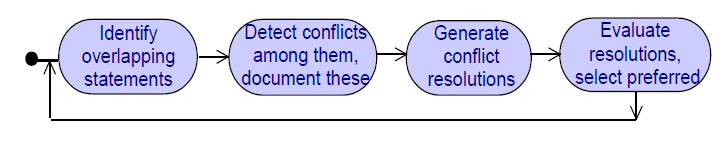
\includegraphics[width=0.5\textwidth]{img/requirements/conflicts.png}
    \caption{Managing conflicts}
    \label{fig:conflicts}
\end{figure}
Analizzando nel dettaglio la figura \ref{fig:conflicts} abbiamo:
\begin{enumerate}
    \item Nella fase di sovrapposizione/overlap indichiamo il riferimento a
          termini o fenomeni comuni.
    \item La fase di riconoscimento può essere fatta informalmente, tramite
          euristiche sulle categorie dei requisiti in conflitto, o formalmente. Il
          riconoscimento deve essere documentato per una successiva risoluzione e analisi
          dell'impatto. Si usano strumenti come l'interaction matrix che presenta su
          righe e colonne gli statement e negli incroci indica:
          \begin{itemize}
              \item 1 per il conflitto
              \item 0 per nessun overlap
              \item 1000 per overlap senza conflitto
          \end{itemize}
          Avendo, per ogni statement $S_i$, indicando con $S_i$ la riga/colonna
          corrispondente (sono uguali):
          \begin{equation}
              conflicts(S_i) = \left(\sum_{s \ \in \ S_i} s \right) \mod 1000
          \end{equation}
          \begin{equation}
              nonConflictingOverlaps(S_i) = \left\lfloor \sum_{s \ \in \ S_i} s / 1000 \right\lfloor
          \end{equation}
    \item La terza fase è strutturata nel seguente modo:
          \begin{itemize}
              \item Esplorare prima più risoluzioni, generate tramite tecniche
                    di elicitation e usando tattiche di risoluzione dei conflitti:
                    \begin{itemize}
                        \item Evitare condizioni a contorno
                        \item Ripristinare statement in conflitto
                        \item Indebolire gli statement in conflitto
                        \item Non considerare statement a bassa priorità
                        \item Approfondire source e target del conflitto
                    \end{itemize}
              \item Confrontare, selezionare e concordare il preferito poi.
          \end{itemize}
          Si trasformano quindi statement in conflitto (e parti coinvolte) in nuovi requisiti.
    \item Nella quarta fase si usano vari criteri per la scelta:
          \begin{itemize}
              \item Contributo a requisiti non funzionali critici.
              \item Contributo alla risoluzione di altri conflitti e rischi.
              \item Applicazione dei principi di risk analysis.
          \end{itemize}
\end{enumerate}

La parte di \textbf{Requirements prioritization} consiste nel fornire ai vari
requisti una prioritizzazione, per vari scopi:
\begin{itemize}
    \item Risoluzione dei conflitti.
    \item Limitazioni delle risorse.
    \item Sviluppo incrementale.
    \item Ri-pianificazione a causa di problemi imprevisti.
\end{itemize}
e si hanno vari principi per una buona riuscita della stessa, che può essere
svolta tramite:
\begin{enumerate}
    \item \textbf{Livelli ordinati} di uguale priorità, in un piccolo numero.
    \item \textbf{Livelli relativi} come ad esempio \textit{maggiore di}.
    \item \textbf{Requisiti comparabili}: stessa granularità, stesso livello di
          astrazione.
    \item \textbf{Requisiti non mutuamente dipendenti}.
    \item Un \textbf{accordo} con i vari partecipanti e stakeholder.
\end{enumerate}
Per i primi tre posso usare una tecnica sistematica basata su diversi step:
\begin{itemize}
    \item Stimare il contributo relativo di ogni richiesta al valore del progetto.
    \item Stimare il contributo relativo di ciascuna richiesta al costo del progetto.
    \item Tracciare il diagramma valore-costo.
\end{itemize}

Si usa quindi la tecnica AHP dalla Decision Theory dove si cerca di capire in che
proporzione ogni requisito $R_i$ contribuisce al criterio $crit$, che sarà prima
il valore, $crit = value$, e poi il costo, $crit = cost$. Si hanno quindi due step:
\begin{enumerate}
    \item Si usa la comparison matrix stimando i contributi di ogni requisito sul
          criterio da studiare. Avendo $N$ requisiti:
          \begin{equation}
              R_{i, j} = \frac{1}{R_{i, j}}, \ \ \ \text{se} \ 1 \leq i, j\leq N
          \end{equation}
    \item Si determina quanto questo si distribuisce tra tutti i requisti, tramite
          gli autovalori della matrice. Inoltre le colonne vengono normalizzate tramite:
          \begin{equation}
              R_{i, j} = \frac{R_{i, j}}{\sum_i R_{i, j}}
          \end{equation}
          e aggiungendo la media sulle righe per valutare il contributo del requisito
          sul criterio.
\end{enumerate}
AHP permette di assicurare stime e rapporti consistenti.
\subsection{Specification \& documentation}
In questa fase si documentano in modo preciso i requisiti scoperti. Si descrivono
in modo preciso le feature e i concetti rilevanti per il progetto. Nel dettaglio
si definiscono in modo preciso:
\begin{itemize}
    \item Obiettivi, concetti, proprietà di dominio rilevanti, requisiti di
          sistema/software, ipotesi, responsabilità
    \item La motivazione delle opzioni scelte
    \item Un'indicazione sulle varianti e sulle evoluzioni previste
\end{itemize}

Il documento deve avere una struttura coerente. Tale documento è detto
\textbf{Requirements Document} (RD). Qualora i requisti siano stati messi online
si procede alla costruzione di un database che tiene traccia dei requisti. In ogni
caso il contenuto deve essere accessibile e comprensibile da tutte le parti
interessate, aggiungendo spesso in allegato anche costi, workplan e piani di delivery.
Bisogna capire come effettivamente documentare i requisiti.

La prima opzione è l'utilizzo del linguaggio naturale in modo svincolato. Si ha
una forte espressività ma, in assenza di regole sulla scrittura si rischia di
produrre una sorta di romanzo, producendo qualcosa di poco gestibile. Il linguaggio
naturale inoltre può nascondere ambiguità. Usando il linguaggio naturale privo
di vincoli si hanno quindi rischi ma si può usare un linguaggio naturale strutturato,
per ottenere tale linguaggio si introducono quindi due tipi di regole:
\begin{enumerate}
    \item \textbf{Local rules}, che riguardano la scrittura del singolo requisito.
    \item \textbf{Global rules}, che riguardano le regole sulla scrittura
          dell'intero documento e sull'insieme dei requisti.
\end{enumerate}
Abbiamo però alcune regole stilistiche generali:
\begin{itemize}
    \item Scrivere pensando a chi deve leggere, che deve essere ben identificato.
    \item Spiegare cosa stiamo per scrivere prima di specificarlo nel dettaglio.
    \item Prima motivare le scelte, indicare le scelte e poi fare un sommario delle stesse.
    \item Assicurarsi che ogni concetto usato nei requisiti sia stato prima ben definito.
    \item Chiedersi se quanto scritto è comprensibile e rilevante.
    \item Per ogni frase/elemento del documento indicare uno e un solo requisito
          o assunzione o proprietà di dominio, evitando di mischiare troppe cose.
    \item Scrivere frasi brevi.
    \item Distinguere ciò che è obbligatorio da ciò che è desiderabile.
    \item Evitare acronimi non necessari ed evitare l'abuso del gergo informatico.
    \item Usare esempi esplicativi.
    \item Usare diagrammi o illustrazioni quando utile.
\end{itemize}

In termini di \textit{local rules} si hanno dei template per scrivere i requisiti,
usando anche un solo standard per tutti i requisti. Un esempio di template potrebbe contenere:
\begin{itemize}
    \item Identificatore del requisito, con uno schema di naming significativo.
    \item Categoria del requisito (funzionale, assunzione $\dots$).
    \item Specifica del requisito (usando le regole stilistiche).
    \item Criterio di fit o test di accettazione, il quale è usato quindi per
          quantità/concetti misurabili, essendo critico quindi per requisiti non funzionali.
    \item Fonti di elicitazione.
    \item Motivazioni.
    \item Interazioni con altri requisti (contribuzioni, dipendenze e conflitti).
    \item Livello di priorità.
    \item Livelli di stabilità (per indicare le chance di cambiamenti).
\end{itemize}
Per le \textit{global rules} si ha una forma standard data da IEEE std-830, il
più diffuso. Si hanno varie macro-categorie a loro volta suddivise in:
\begin{enumerate}
    \item \textit{Introduzione}: si specifica anche quale parte del documento
          interessi ai vari stakeholder:
          \begin{enumerate}
              \item Motivazioni del documento.
              \item Scopo del prodotto.
              \item Definizioni, acronimi, sigle e abbreviazioni.
              \item Reference, fonti di elicitazione.
              \item Overview dell'organizzazione del documento.
          \end{enumerate}
    \item \textit{Descrizione generale}
          \begin{enumerate}
              \item Prospettive del prodotto.
              \item Funzionalità principali.
              \item Caratterizzazione degli utenti.
              \item Vincoli generali sull'ambiente (che non possono esse modificati
                    ma con i quali si deve integrare il prodotto).
              \item Assunzioni sul prodotto e dipendenze del prodotto.
              \item Ripartizione dei requisti.
          \end{enumerate}
    \item \textit{Requisiti specifici} usando magari il template visto prima. Si
          hanno quindi varie categorie di requisiti che articolano le varie sezioni del capitolo:
          \begin{enumerate}
              \item Requisiti funzionali, che a sua volta può avere un'organizzazione
                    interna in base a vari fattori.
              \item Requisiti per l'interfaccia esterna.
              \item Requisiti per le prestazioni.
              \item Vincoli di progettazione.
              \item Attributi di qualità del software
              \item Altri requisiti
          \end{enumerate}
    \item Appendice.
    \item Indice.
\end{enumerate}

Una variante per il template VOLERE dove si hanno sezioni esplicite per proprietà
del dominio, costi, rischi, piano di lavoro di sviluppo etc$\dots$
\subsubsection{Diagrammi}
Si hanno anche opzioni aggiuntive oltre al linguaggio naturale. Una prima alternativa
sono i diagrammi, dove si ha una notazione semi-formale, in quanto si ha una sintassi
formale essendo i vari diagrammi formalmente definiti ma l'interpretazione degli
stessi può comunque essere ambigua.

I diagrammi sono utili per complementare quanto scritto in linguaggio naturale, che
spesso risulta troppo complesso e articolato. Un diagramma può semplificare quanto
scritto e rappresentare il tutto in modo compatto. L'uso di diagrammi permette
di ottenere un metodo di comunicazione più semplicemente e viene usato per aspetti
specifici del sistema. Si ha comunque la stessa ambiguità di interpretazione
che si aveva nei linguaggi naturali.
\paragraph{Problem diagram}
Un primo esempio di digramma utilizzato è il \textbf{problem diagram}
\ref{fig:problemDiagram}, il quale
descrive i requisiti a livello di sistema.

In questo diagramma si descrive il problema che si vuole risolvere, mostrando le
componenti del sistema e le loro interazioni. Si può specificare testualmente un
requisito e riferirlo alle componenti del sistema citate nel requisito, che è
posto in un ellisse tratteggiato. Posso avere riferimenti e vincoli sulle
componenti a partire dal requisito. Tutte le interazioni sono decorate con gli
eventi che sono rilevanti per l'interazione con il produttore dell'evento indicato
tramite le maiuscole e il nome dell'evento, a loro volta separati da “!”.

Ogni componente del sistema è indicata tramite un rettangolo in cui è presente
una doppia linea a sinistra. Il sistema comunica con diversi elementi dell'ambiente,
indicati da rettangoli.

Con questo tipo di diagramma si cattura il contesto del requisito, legandolo
componenti dell'ambiente e componenti del sistema, tramite specifici eventi.
Si identificano a colpo d'occhio gli elementi rilevanti per un certo requisito.
\begin{figure}[!ht]
    \centering
    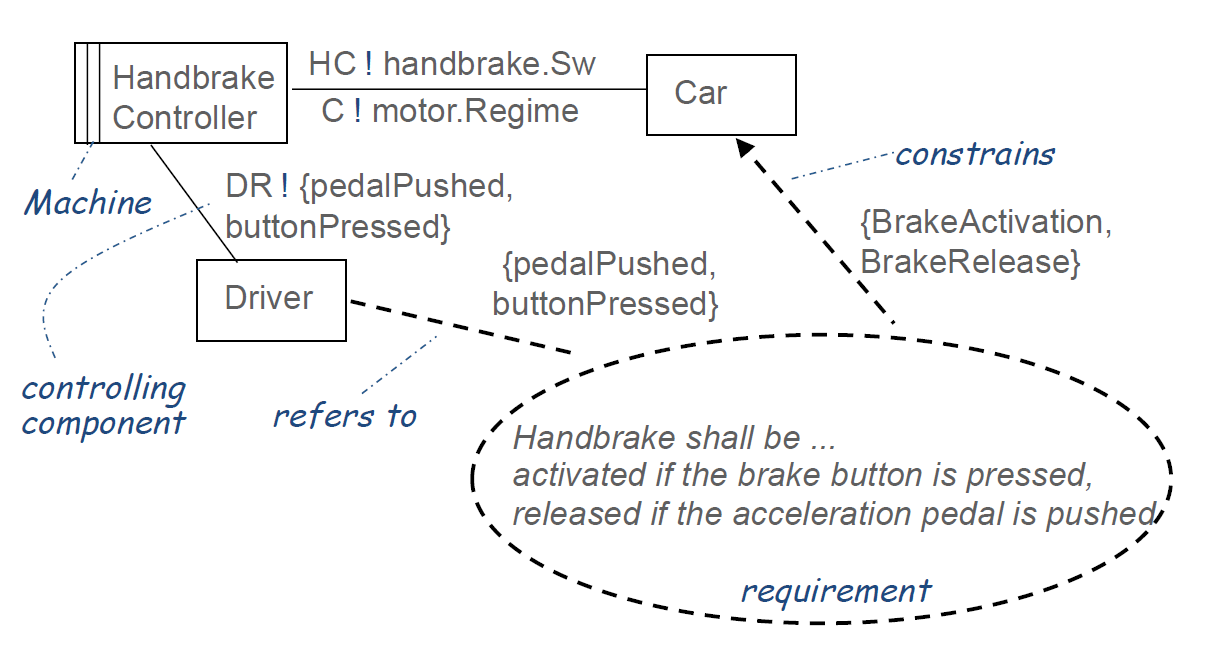
\includegraphics[width = \textwidth]{img/requirements/PD.png}
    \caption{Esempio di Problem Diagram}
    \label{fig:problemDiagram}
\end{figure}

Questa rappresentazione può prendere la forma di veri e propri pattern detti
\textbf{problem pattern} per semplificare la rappresentazione. Si ottengono i
\textbf{frame diagrams}, che hanno la stessa rappresentazione dei problem diagram
con la differenza che si ha qualche informazione in più:
\begin{itemize}
    \item \textbf{Tipo di componente}, indicato con un quadratino in basso a
          destra nel rettangolo della componente, specificato da una lettera:
          \begin{itemize}
              \item C: causal, causa-effetto
              \item B: biddable, non predicibile
              \item X: lexical, lessicale, specifica artefatti
          \end{itemize}
    \item \textbf{Tipo di evento} (posto) dopo il “!” sopra descritto, specificato
          da una lettera:
          \begin{itemize}
              \item C: causal, diretta conseguenza di altri eventi
              \item E: event, che non sono diretta conseguenza ma che sono prodotti
                    in modo spontaneo
              \item X: lexical, dati che vengono utilizzati per produrre qualcosa
          \end{itemize}
\end{itemize}
Tali pattern vengono istanziati nei vari casi specifici.
\paragraph{Diagrammi ER}
Un altro diagramma tipico è quello ER per specificare entità che entrano in gioco
in certi aspetti dei requisiti, specificandole in modo schematico. Si usano anche
diagrammi di dominio, di classe etc$\dots$, non descrivendo più comportamenti
ma strutture, domini etc$\dots$
\paragraph{Diagrammi SADT}
I \textbf{SADT diagrams} permettono di specificare il comportamento di alcune
attività scomponendolo e aggiungendo varie informazioni. Possiamo avere due tipi
di diagrammi:
\begin{enumerate}
    \item \textbf{Actigram} \ref{fig:actigram}: sono di tipo \textit{activity-driven}
          e si concentrano sulle attività e sul mostrare le dipendenze tra le attività
          in termini di dati. Le attività sono indicate dentro rettangoli e si hanno
          una serie di frecce che a seconda della direzione variano il significato:
          \begin{itemize}
              \item $\to$ per l'input di dati.
              \item $\gets$ per l'output di dati.
              \item $\downarrow$ per il data/event controlling, ovvero dati o
                    eventi che controllano il comportamento dell'attività, sono magari
                    aspetti di configurazione etc$\dots$ che influenzano l'attività
              \item $\uparrow$ per l'unità che processerà l'attività, questa può
                    essere opzionale.
          \end{itemize}
          \begin{figure}[!ht]
              \centering
              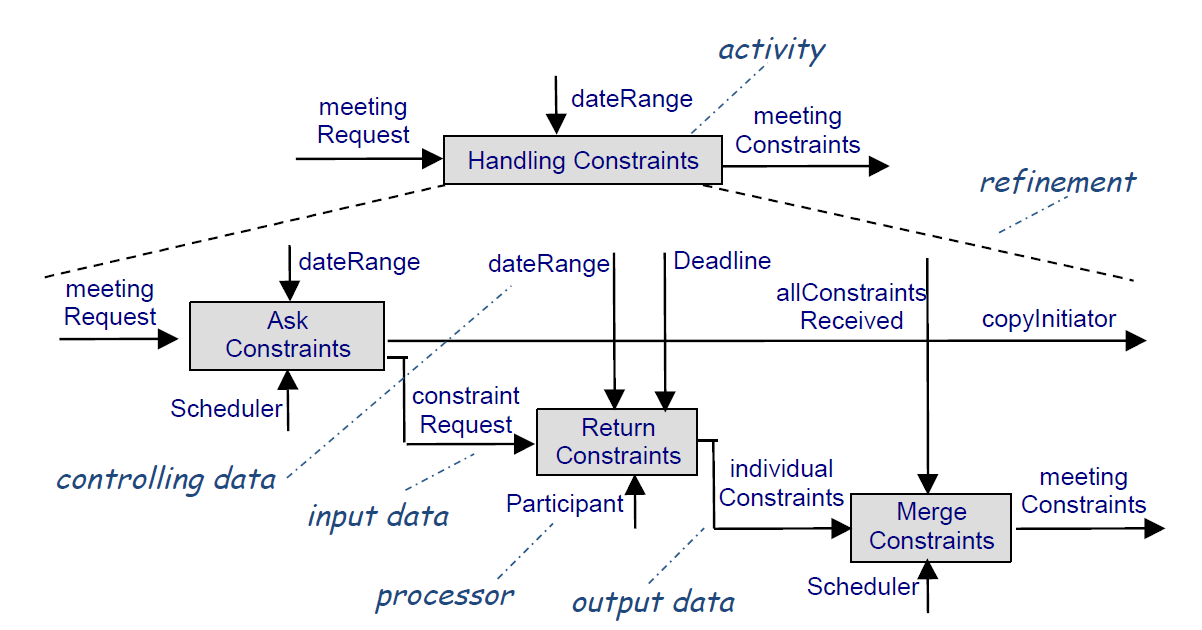
\includegraphics[width = \textwidth]{img/requirements/actigram.png}
              \caption{Actigram}
              \label{fig:actigram}
          \end{figure}
    \item \textbf{Datagram} \ref{fig:datagram}: sono di tipo \textit{data-driven},
          si concentrano sui dati e mostrano le dipendenze tra i dati in termini di
          attività. I dati sono indicate dentro rettangoli e si hanno una serie di frecce
          che a seconda della direzione variano il significato:
          \begin{itemize}
              \item $\to$ per l'input di attività che producono il dato.
              \item $\gets$ per l'output di attività verso le quali serve il dato.
              \item $\downarrow$ per le attività di validazione del dato.
              \item $\uparrow$ per le risorse necessarie a memorizzare e gestire il dato.
          \end{itemize}
          \begin{figure}[!ht]
              \centering
              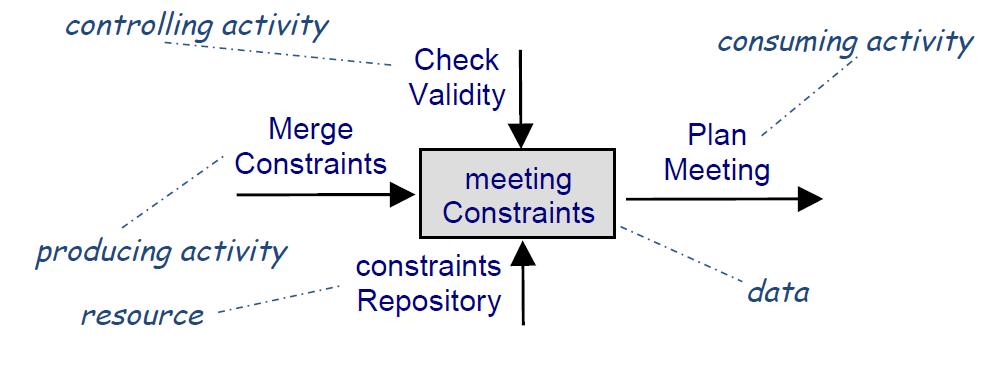
\includegraphics[width=\textwidth]{img/requirements/datagram.png}
              \caption{Datagram}
              \label{fig:datagram}
          \end{figure}
\end{enumerate}
La coerenza tra di due diagrammi è fondamentale avendo una rapporto di dualità
tra essi quindi i dati e le attività presenti in uno devono apparire anche nell'altro.

Questo strumento si prestano a documentare workflow molto semplici. In ogni caso:
\begin{itemize}
    \item Ogni attività deve avere un input e un output.
    \item Tutti i dati devono avere un produttore e un consumatore.
    \item I dati I/O di un'attività devono apparire come dati I/O delle sotto-attività.
    \item Ogni attività in un datagramm deve essere definita in un actigramma.
\end{itemize}
\paragraph{Use case Diagram}
Un altro diagramma classico è lo \textbf{use case diagram} per visualizzare i
requisiti identificati, che prendono forma di casi d'uso con gli attori che partecipano
allo svolgimento dei requisiti.
\paragraph{Event trace diagrams}
Un altro strumento utile nella definizione di workflow è l'\textbf{event trace diagrams}
\ref{fig:etd}, ovvero i diagrammi di sequenza. Se ne hanno vari tipi con sintassi
più o meno ricche ma in generale si hanno $N$ elementi che partecipano all'esecuzione
che viene mostrata visualmente tramite richieste e risposte, sincrone o meno,
che vengono indicate cronologicamente dall'alto al basso.
\begin{figure}[!ht]
    \centering
    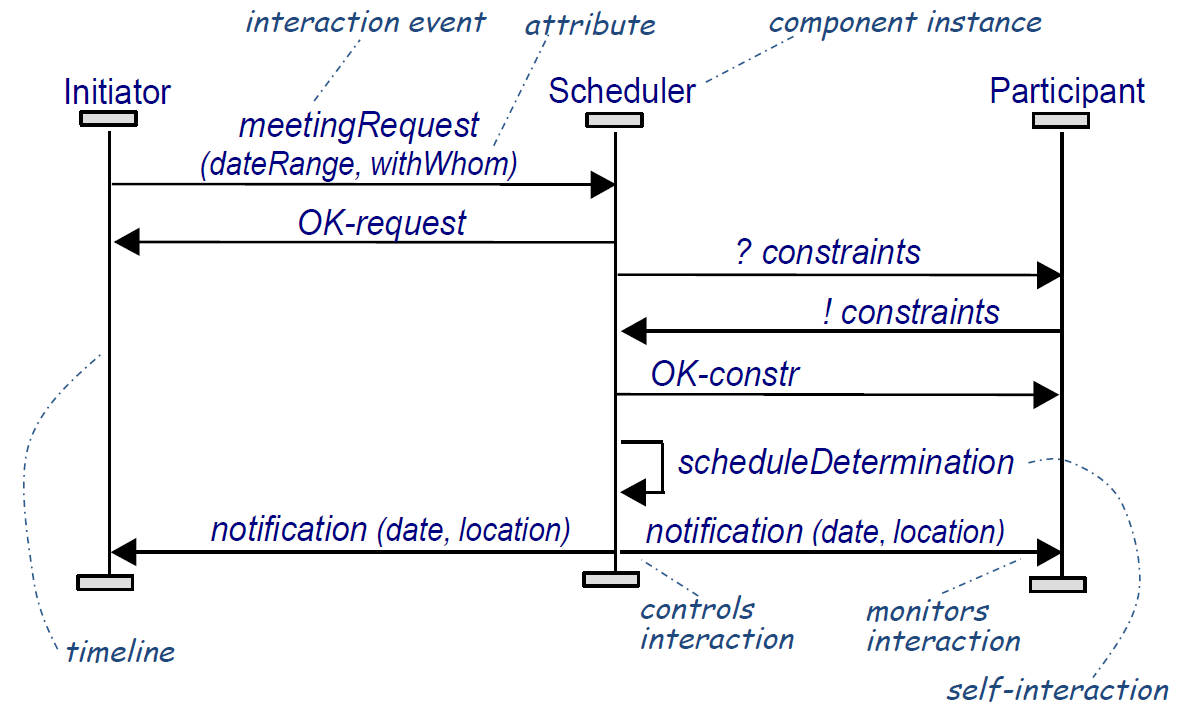
\includegraphics[width=\textwidth]{img/requirements/etd.png}
    \caption{Event trace diagrams}
    \label{fig:etd}
\end{figure}
Questa visualizzazione compatta aiuta nel momento in cui il linguaggio naturale
diventa troppo complesso e verboso per spiegare una certa sequenza di azioni.
\paragraph{State machine diagram}
Un altro diagramma usato è lo \textbf{state machine diagram} \ref{fig:smd} per
mostrare in quali stati un particolare elemento si trova e quali transizioni/eventi
modificano i suoi stati. Questi diagrammi sono utili in quanto in modo compatto
rappresentano il ciclo di vita di una certa componente, facilitando la creazione
del sistema.
\begin{figure}[!ht]
    \centering
    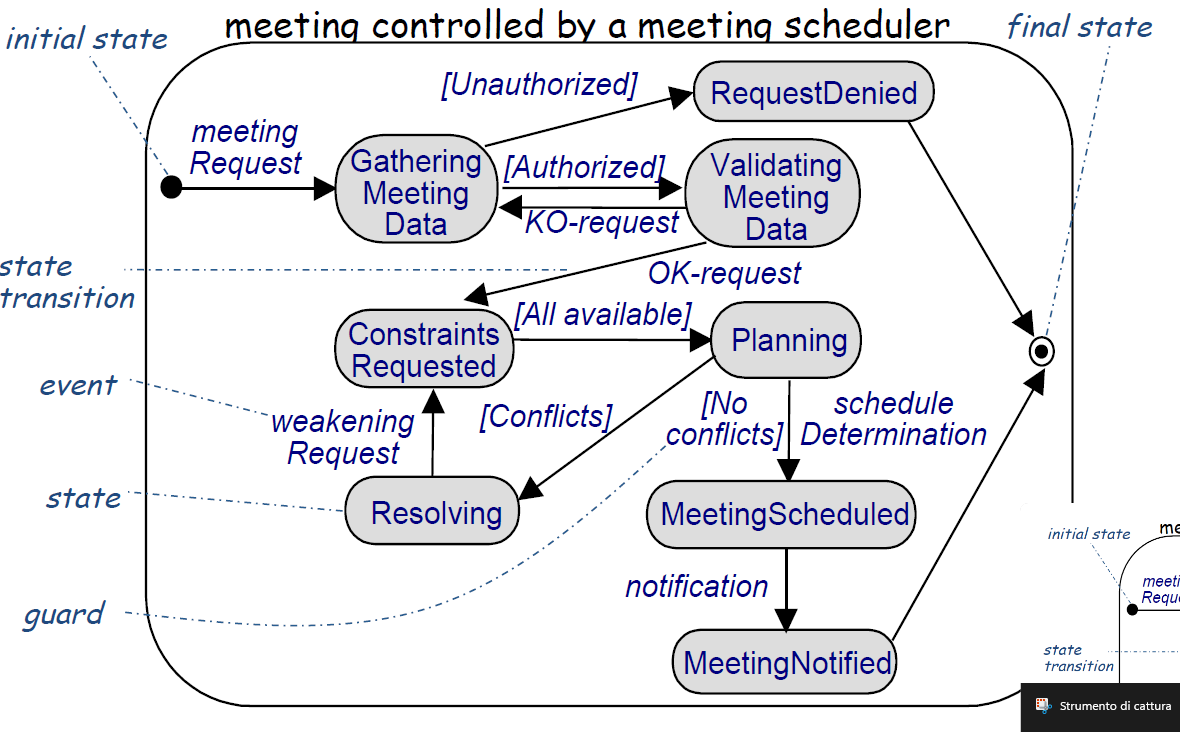
\includegraphics[width=\textwidth]{img/requirements/smd.png}
    \caption{State machine diagram}
    \label{fig:smd}
\end{figure}
\paragraph{R-net diagram}
Come altro diagramma abbiamo il \textbf{R-net diagram} che permette di mostrare
come reagisce un sistema in base ad un certo stimolo. È quindi un albero che parte
con uno stimolo, dopo il begin, posto in un esagono e si sviluppo in base alle
varie alternative in corrispondenza di punti di decisione (indicati come pallini).
Nei rettangoli si hanno le azioni che sono svolte in conseguenza allo stimolo.

I diagrammi sono tra loro complementari ma hanno anche delle intersezioni tra
loro e anche con il testo e tutto deve comunque restare coerente. Si rischia di
introdurre inconsistenze.

Si hanno alcune regole di consistenza per i diagrammi che vengono usate da diversi
strumenti per verificare la consistenza tra i vari diagrammi.

A questo punto è doveroso citare uno degli standard per la modellazione di
diagrammi: \textbf{Unified Modeling Languag}e (UML). Al suo interno si hanno, con regole di coerenza tra essi:
\begin{itemize}
    \item class diagrams
    \item use case diagrams
    \item sequence diagrams
    \item state diagrams
\end{itemize}

In conclusione i diagrammi hanno il pro di essere in grado di dare una buona panoramica
e struttura/comportamento, facile da trasmettere e comprendere, di aspetti importanti.
Sono inoltre supportati da vari tool di analisi.

Il contro è sempre la specifica ambigua semi-formale che può anche limitare l'analisi
degli stessi. Inoltre si concentrano solo su aspetti funzionali e strutturali.

Si hanno anche gli statechart per la descrizione di sistemi paralleli che usano
la semantica interleaving ovvero per 2 transizioni che si attivano nello stesso
stato, una viene presa dopo l'altra, in modo non deterministico.
\subsubsection{Alternative alla specifica semi-formale}
Si ha quindi in generale la necessità di una semantica formale per aspetti
mission-critical e la cosa non viene garantita dai diagrammi ma si hanno linguaggi
apposta (e diagrammi apposta) la cui creazione/gestione/documentazione è assai
costosa per cui vengono usati solo in casi estremamente specifici. Approfondiamo
quindi questi linguaggi e questa notazione.

Si parla sia di sintassi che di semantica. Tali definizioni formali permettono
che il compilatore sia in grado di processare tali specifiche. Si ha quindi un
livello di precisione alto e non si ha ambiguità, permettendo analisi di consistenza
e coerenza delle specifiche.

Una sintassi/semantica formale è quella data dalla logica proposizionale e dalle
formule ben formate. Si ha quindi un linguaggio basato sui connettori logici e
sulle regole per avere formule ben formate.

Ogni statement può quindi essere interpretato con il valore di verità con le
regole definite dalla logica e dalle tabelle di verità. Si vede quanto produrre
tutto questo per un progetto enorme risulti costoso. Vengono quindi usate le
classiche regole di inferenza. Si usa anche la logica predicativa del primo ordine.

Un altro strumento usato è la logica temporale con l'aggiunta dei connettivi temporali.

Si ha un approccio formale anche su specifiche state-based dove si specifica in
modo formale cosa sia l'insieme degli stati che il sistema può attraversare e
come delle operazioni modificano lo stato.

Si usano linguaggi come $Z$ basati sulla teoria degli insiemi. Ogni stato è
caratterizzato da pre e post condizioni e si studiano le regole in termini di
invarianti che lo stato deve soddisfare.

Con Z si producono schemi dove si specifica un certo elemento, gli attributi di
stato con P che indica l'insieme delle parti che precede il tipo. Si ha poi un
invariante per gli attributi che definisce l'elemento. Si ha quindi una caratterizzazione
basata sulla teoria degli insiemi. Si hanno sia tipi primitivi che strutturati.
Per definire invece le modifiche che portano a nuovi stati.

Sopra si hanno tutti gli elementi coinvolti nell'operazione. La prima linea della
parte sotto è per le precondizioni, quella sotto per le postcondizioni, entrambe
con la notazione insiemistica. Gli elementi sono inoltre così decorati:
\begin{itemize}
    \item stateVar?:Type indica una variabile di input
    \item stateVar':Type indica una variabile di output mutevoli
    \item stateVar!:Type indica una variabile di output esterne e non mutevoli
    \item $\Delta$ schema indica che si ha una modifica delle variabili importate
          dallo schema
    \item $\Xi$ schema indica che non si ha una modifica delle variabili importate
          dallo schema
\end{itemize}

Il cambiamento di stati ben definito diventa studiabile e simulabile, studiando
lo spazio di comportamenti del sistema a questo livello di astrazione, individuando
problemi che porterebbero alla correzione di requisiti. Si può avere anche
l'inclusione di più schemi. Con questa specifica state-based si hanno vari pro:
\begin{itemize}
    \item automazione semplice grazie a logica, matematica discreta, studio degli
          invarianti etc$\dots$
    \item ottimi meccanismi di strutturazione per comporre unità e strutture
          stati complessi
    \item permette l'analisi automatica: type checking, consistency checking,
          etc$\dots$
\end{itemize}

Di contro non permette di studiare altro se non aspetti funzionali e non ha
un'historical referencing.

Si ha anche una specifica algebrica per formalizzare le leggi che compongono le
operazioni, viste come funzioni matematiche senza esplicita nozione di stato.
Si ha invece un system history avendo una “traccia” delle operazioni.

Si hanno tipi di dato astratti, parametrizzazione, equazioni condizionali e funzioni
parziali. Si hanno tre tipi di operazione:
\begin{enumerate}
    \item modifiers, per produrre qualsiasi istanza di concetto mediante composizione
          con altri modifier
    \item generators, ovvero un sottoinsieme minimo di modifiers per generare
          qualsiasi istanza di concetto con un numero minimo di composizioni
    \item obsevers, per ottenere informazioni pertinenti su qualsiasi istanza di
          concetto
\end{enumerate}

Spesso si hanno funzioni ricorsive.

Come vantaggi si hanno:
\begin{itemize}
    \item analisi automatica efficiente
    \item specifiche eseguibili
    \item ricchi meccanismi di strutturazione (import, ereditarietà $\dots$)
\end{itemize}

Di contro si ha una limitata potenza espressiva (solo equazioni senza historical
referencing) e una forte vicinanza alla programmazione (comportando difficoltà
di validazione in caso, ad esempio, di ricorsioni).

Tendenzialmente i limiti della notazione formale sono sempre questi (oltre alla
difficoltà di lettura/scrittura), anche se permette alta precisione, pochi difetti
di specifica, analisi sofisticata (anche automatica), generazione di artefatti
come test cases, codice etc$\dots$.

Ricapitolando:
\begin{itemize}
    \item il linguaggio naturale “puro” non è un'opzione
    \item il linguaggio naturale strutturato è quello più usato
    \item i diagrammi sono un'ottima aggiunta al linguaggio naturale
    \item la notazione formale è usata in rare circostanze
\end{itemize}
\subsection{Validation \& verification}
Siamo quindi all'ultima delle quattro fasi, dove bisogna validare i requisiti.
Si hanno vari approcci per validare la qualità dei requisiti.
\subsubsection{Analisi e revisione dei singoli requisiti}
Questo è sempre applicabile ma va fatto manualmente impiegando molto tempo. La
prima operazione consiste nel ricercare errori nel Requirements Document. Spesso
questi sono gli errori più numerosi e pericolosi e possono avere varia natura:
\begin{itemize}
    \item Omissione
    \item Contraddizione
    \item Inadeguatezza
    \item Ambiguità
    \item Incommensurabilità
    \item Rumore
    \item Eccesso di specificità
    \item Scarsa struttura
    \item Opacità
\end{itemize}
Bisogna quindi individuare quanti più problemi possibili nel Requirements Document,
validarli (vedendo se le informazioni utili sono necessarie), verificarli (vedendo
se sono completi e consistenti) e confermare non ambiguità, misurabilità,
fattibilità, buona struttura, etc$\dots$

Bisogna quindi fare il report dei problemi, analizzarne la causa e correggerli.
Questa operazione viene fatta selezionando personale che ispeziona il Requirements
Document individualmente per poi confrontare le opinioni. Tali persone possono
essere interne ai project members o recensori esterni. Questo viene spesso fatto
anche per il codice sorgente e quindi si è mostrato che è empiricamente utile
anche per le revisioni del Requirements Document.

La revisione può essere effettuata in vari modi:
\begin{itemize}
    \item \textbf{Free mode}: senza direttiva su cosa cercare e dove.
    \item \textbf{Checklist-based}: indicando una lista di cose da controllare.
    \item \textbf{Process-based}: dove si hanno ruoli specifici, procedure dettagliate,
          tecniche di analisi etc$\dots$, rendendo questa la modalità più efficace.
\end{itemize}
Il report deve essere fatto in modo informativo e accurato, senza opinioni o
commenti offensivi (anche se può essere lasciato uno spazio per i commenti liberi).
Ovviamente le revisione deve essere fatta possibilmente da personale diverso da
quello che scrive il Requirements Document e tale personale deve rappresentare
tutti gli stakeholder con le varie conoscenze pregresse.

A livelli di tempo il controllo deve essere effettuato ne troppo presto ne troppo
tardi ma con incontri ripetuti per ottenere la massima efficacia.

Ci si deve inoltre concentrare sulle parti più critiche, che devono essere meglio
analizzate. Dal punto di vista delle checklist se ne hanno diverse:
\begin{itemize}
    \item \textbf{Defect-driven}: lista dei difetti tipici, strutturate tramite
          un elenco di domande generiche.
    \item \textbf{Quality-specific}: lista più specializzata di quella defect-driven,
          specializzandosi su requisiti non funzionali.
    \item \textbf{Domain-specific}: lista specializzata nei concetti e nelle
          operazioni di dominio per aiutare nella ricerca dei difetti:
    \item \textbf{language-based}: lista specializzata nei costrutti legati ai linguaggi.
          In questa parte si analizzano anche i diagrammi, si analizzando anche
          linguaggi di specifica come Z.
\end{itemize}
Si usano anche delle \textbf{checking decision tables} che hanno in input $N$
condizioni booleane ($\{T, F\}$) e una serie di eventi che si hanno in conseguenza
allo stato delle condizioni, specificando se accadono o meno. Si ha che se il
numero di combinazione dei vari casi specificati dalle condizioni in input è minore
$2^N$ (se ho meno colonne del dovuto nella tabella di verità) allora mancano dei
casi da analizzare mentre se è maggiore si hanno dei casi ridondanti.

Questo tipo di analisi è quindi applicabile potenzialmente alla ricerca di ogni
difetto (anche se non si ha garanzia di riconoscerli tutti, per quanto critici,
anche se con un mix delle tecniche spiegate si raggiungono ottimi risultati).
I costi restano elevati sia in termini monetari che di tempo.
\subsubsection{Interrogare il database delle specifiche}
Questo, a livello superficiale, può essere fatto in modo automatico ma è appunto
un check parziale. Questa tecnica è specifica per casi particolari, dove le
specifiche sono memorizzate in un database. Le query acquisiscono controlli per
la coerenza strutturale intra o inter-diagrammi e tali query possono essere generate
a partire dall'ER. Si parla anche di press-button mode quando si ha una lista
di query prescritte per la violazione delle regole di coerenza standard.
\subsubsection{Usare le specification animation}
Sono ottime per i non esperti per identificare i problemi ma sono limitate alle
specifiche “eseguibili”, consentendo quindi solo un check parziale. Si vuole
verificare l'adeguatezza dei requisiti rispetto alle effettive necessità. Si
hanno due approcci tipici:
\begin{enumerate}
    \item Mostrare una vera interazione cono lo scenario. In questo caso gli
          strumenti di “promulgazione” possono essere utilizzati sul diagramma NET ma
          ovviamente si ha il problema del range di copertura dei problemi dato dallo
          scenario.
    \item Usare tool per l'animazione delle specifiche. Si procedere generando
          un modello eseguibile e si procede alla simulazione (provvedendo a stimoli e
          vedendo il risultato) per poi raccogliere il feedback dell'utente. Si può avere:
          \begin{itemize}
              \item Formato testuale, con comandi di input e poi esecuzione.
              \item Formato a diagrammi, con un input che comporta l'evoluzione
                    di parti del diagramma.
              \item Scena vera e propria con pannelli per l'input e scene animate
                    nell'ambiente scelto.
          \end{itemize}
\end{enumerate}
In ogni caso si ha un approccio model-based, si parla infatti di model-driven
development (sviluppando fin dall'inizio modellando il comportamento del software),
e si hanno vari tool per i vari linguaggi di specifica (SCR, LTSA etc$\dots$).

Tra i pro si hanno:
\begin{itemize}
    \item È modo migliore per verificare l'adeguatezza rispetto ai bisogni reali,
          all'ambiente reale
    \item Permette la facile interazione con gli stakeholder secondo la filosofia
          WYSIWYC (What You See Is What You Check)
    \item Estendibile per animare controesempi generati da altri strumenti.
    \item Le animazioni possono essere riusate per altri scenari.
\end{itemize}
Si hanno anche contro:
\begin{itemize}
    \item Si richiede un'attenta progettazione degli scenari che possono presentare
          problemi e non si ha garanzia di non trascurare problemi critici.
    \item Necessita specifiche formali.
\end{itemize}
\subsubsection{Check formale}
Questo permette di individuare un ottimo range di problemi ma richiede la notazione
formale, costosa, ed esperti. Si possono avere check sintattici per il linguaggio
(di specifica come Z) usato (syntax checking, type checking, static semantics
checking, le variabili utilizzate devono essere dichiarate e inizializzate,
devono essere utilizzate nello scope corretto etc$\dots$, circularity checking,
con il check delle postcondizioni etc$\dots$). Si può avere anche un check di
completezza e consistenza grazie al linguaggio e la verifica di proprietà:
\begin{itemize}
    \item Algoritmiche tramite model checking, per controllare se un modello di
          comportamento soddisfa un requisito, una proprietà di dominio o un presupposto,
          cercando violazione delle varie proprietà e generando eventuali controesempi
          o comunque specifiche della violazione (fattori utili nel debugging).
          Si possono controllare:
          \begin{itemize}
              \item Raggiungibilità, tramite un grafo di raggiungibilità
              \item Proprietà di safety, producendo controesempi
              \item Proprietà di liveness, che comporta che una condizione potrebbe
                    non essere mai raggiunta in caso di risposta negativa del check
          \end{itemize}
          I pro del model checking sono:
          \begin{itemize}
              \item Check completamente automatici
              \item Ricerca esaustiva che porta a non tralasciare alcun difetto
              \item L'uso di controesempi può rivelare errori sottili, difficili
                    da individuare altrimenti
              \item È facile da abbinare agli animators per visualizzare le tracce
              \item È sempre più usato per progetti mission critical
          \end{itemize}
          Ma si hanno anche dei contro:
          \begin{itemize}
              \item Si rischia di avere un'esplosione combinatoria degli stati da
                    analizzare comportando l'impossibilità di essere eseguito per
                    sistemi molto grossi.
              \item I controesempi possono essere complessi da capire e mostrano
                    solo i sintomi dei problemi, non le cause.
          \end{itemize}
    \item \textbf{Deduttive tramite theorem proving}. Il theorem proving viene
          usato per generare nuove specifiche tramite le regole di inferenza della logica.
          Si studiano le conseguenze logiche delle specifiche evidenziando eventuali
          inconsistenze in un processo generalmente iterativo per:
          \begin{itemize}
              \item Fornire, accettare o rifiutare i lemmi.
              \item Suggerire strategie di prova.
          \end{itemize}
          Si hanno diversi pro:
          \begin{itemize}
              \item solidità e completezza del sistema formale utilizzato avendo
                    che ogni conclusione è corretta e che ogni conclusione corretta è derivabile
              \item mostra specifiche incoerenti, conseguenze inadeguate
              \item può essere usato per sistemi molto grandi, gestendo una gran
                    mole di dati tramite l'induzione
          \end{itemize}
          ma si hanno ovviamente dei contro:
          \begin{itemize}
              \item è di uso difficile e richiede personale esperto
              \item non produce controesempi
          \end{itemize}
\end{itemize}
Si hanno, per i check di consistenza quando servizi o comportamenti sono specificati
come relazioni I/O capendo:
\begin{itemize}
    \item se la relazione e una funzione (per isolare eventuali non determinismi)
    \item se la funzione è totale e quindi in grado di specificare ogni input
\end{itemize}
\subsection{Requirements changes}
I cambiamenti dei requisiti sono assai frequenti e quindi vanno gestiti. Si hanno
infatti varie iterazioni delle 4 fasi sopra descritte, formando la spirale.
In primis si hanno cambiamenti organizzativi, nuove normative, nuove opportunità,
tecnologie alternative, priorità e vincoli in evoluzione oltre ad una migliore
comprensione delle caratteristiche, dei punti di forza, dei limiti e dei difetti
del sistema. Un altro aspetto riguarda il problema di gestione delle informazioni,
in merito al mantenimento della coerenza, propagazione delle modifiche, controllo
delle versioni etc$\dots$

La gestione dei cambiamenti di requisito consiste quindi nel processo di anticipazione,
valutazione, accordo e propagazione dei cambiamenti nelle varie parti del
Requirements Document.

Innanzitutto bisogna identificare i cambiamenti probabili, valutare la probabilità
e documentarli al fine di:
\begin{itemize}
    \item Anticipare una risposta adeguata quando si verificherà il cambiamento,
          studiando eventuali dipendenze tra i requisiti.
    \item Progettare l'architettura che rimanga stabile nonostante i cambiamenti.
\end{itemize}
Inoltre, associando livelli di stabilità a gruppi di statement che definiscono le
varie feature. Si punta ad avere un numero di livelli comunque ridotto e di cercare
di permettere la comparabilità, che sia qualitativa e relativa.

Si usano regole euristiche per studiare i probabili cambiamenti, concentrandosi
sui requisiti che è più facile cambino, limitando così i costi. Il livello più
alto di stabilità viene definito per quelle feature presenti in ogni estensione/
variante del sistema. Si ha che aspetti intenzionali e concettuali, così come aspetti
funzionali e obiettivi chiave, sono più stabili di aspetti operazionali e non
funzionali (per esempio la comparsa di una notifica è più stabile del modo in cui
questa viene sviluppata$\dots$ importante è che ci sia la notifica).

La scelta tra varie alternative rende l'oggetto della scelta poco stabile anche
perché tale scelta può essere basata su una conoscenza incompleta, presupposti
volatili o generata da risoluzione di conflitti o contromisure a vari rischi.

Quindi tali requisiti sono poco stabili.

Un altro aspetto essenziale nello studio dell'evoluzione del progetto è legato
alla gestione della \textbf{tracciabilità} (detto anche \textbf{Traceability Management}
(TM)), che non è uno studio semplice nel caso dei requisiti ma torna comodo nel
momento dei loro cambiamenti per gestire il cambiamento dell'intero progetto. Si ha
che un certo aspetto è tracciabile se e solo se si sa perfettamente:
\begin{itemize}
    \item Da dove viene
    \item Perché esiste
    \item Per cosa sarà usato
    \item Come sarà usato
\end{itemize}
Possiamo quindi dire che il TM si occupa di identificare, documentare, recuperare
la logica e l'impatto degli elementi contenuti nel Requirements Document.

Si possono avere anche tracciamenti in merito o obiettivi specifici per determinati
requisiti, valutando l'impatto di eventuali modifiche e studiando come propagare
facilmente i cambiamenti per mantenere la coerenza ad altri elementi
dell'Requirements Document o, “scendendo di livello”, ad oggetti software.

Un aspetto centrale nel TM è rappresentato dai collegamenti di tracciabilità tra
gli elementi del Requirements Document. Tali collegamenti vanno scoperti,
memorizzati ed eventualmente recuperati. Tali collegamenti sono bidirezionali e,
ipotizzando uno schema verticale tra le varie fasi, si hanno:
\begin{itemize}
    \item Accessibilità dal source al target, detta forward traceability
          (che nello schema verticale sono le frecce verso il basso). Il source motiva l'esistenza del target
    \item Accessibilità dal target al source, detta backward traceability
          (che nello schema verticale sono le frecce verso l'alto)
\end{itemize}
All'interno di una stessa fase posso avere anche collegamenti (che in questo caso
non vengono direzionati a differenza dei due appena espressi e sono orizzontali).
Dipendenze tra cambiamenti di fase sono sempre rappresentatati da una linea verticale.

La backward traceability viene usata per stabilire perché un certo elemento sia
lì e da dove viene (anche ricorsivamente) mentre la forward per stabilire dove un
elemento verrà considerato e con quali implicazioni (anche ricorsivamente).
Ricorsivamente perché posso andare indietro/avanti di più step. Bisogna localizzare
e valutare l'impatto dei cambiamenti lungo i collegamenti orizzontali/verticali.

Elencando le varie tecniche TM, per tracciare i vari collegamenti, si hanno:
\begin{itemize}
    \item Cross referencing
    \item Matrici di tracciabilità
    \item Feature diagrams (nel dettaglio quelli con supporto a più variant link
          type)
    \item Database di tracciabilità
    \item Database di modelli di tracciabilità
    \item Tracciabilità Specification-based
\end{itemize}
È comunque un discorso molto complesso, costoso e studiato.

Approfondiamo il cross referencing.

Con questa tecnica si seleziona ogni elemento da tracciare e gli si assegna un
nome unico. Si definisce poi lo schema di indice/tag per collegarli lessicalmente e
si configura un motore di ricerca su tale schema. Si recuperano quindi gli elementi
seguendo le catene di riferimenti incrociati, le cross-reference chains. Un esempio
banale in un documento potrebbe essere specificare che sezione dello stesso documento
andare a guardare per chiarire un certo concetto.

Come pro si hanno:
\begin{itemize}
    \item la leggerezza e la disponibilità
    \item il supporto di ogni livello di granularità (assegnando identificatori
          a ciò che vogliamo)
\end{itemize}
Come contro:
\begin{itemize}
    \item un solo tipo di collegamento, quello lessicale, privo di semantica
    \item informazioni di tracciabilità nascoste
    \item il costo del mantenimento dello schema di indicizzazione (anche se si ha
          un basso costo iniziale)
    \item controllo e analisi limitate
\end{itemize}
In merito alla \textbf{matrice di tracciabilità} abbiamo che essa è la matrice
di adiacenza di un grafo a singola relazione di tracciabilità, detto \textbf{dependency graph}.
In posizione ($i,j$) troviamo 1 se si ha un arco orientato tra l'item $T_i$ e
l'item $T_j$ , 0 altrimenti. Possiamo quindi dire che sulla riga i-sima troviamo
gli elementi che dipendono da $T_i$ e sulla colonna i-sima gli elementi che sono
dipendenza di $T_i$.

Come pro si hanno:
\begin{itemize}
    \item Navigazione backward e forward
    \item Semplice analisi dello schema (ad esempio è semplice identificare un
          ciclo di dipendenza, avendo un ciclo nel grafo)
\end{itemize}
Come contro:
\begin{itemize}
    \item Grafi di grandi dimensioni sono soggetti ad errori oltre ad essere
          difficilmente gestibili
    \item Supportano un solo tipo di relazione
    \item Dovrei creare più matrici per collegamenti tra oggetti con semantiche
          diverse
\end{itemize}
Quest'ultimo contro può essere risolto coi \textbf{feature diagrams} che sono
rappresentazione grafica dei punti in comune e delle varianti del sistema, permettendo
la rappresentrazione compatta di un gran numero di varianti. Avere più varianti
permette di distribuire il sistema con un ampio numero di feature.

Nel diagramma le feature sono rettangoli e possono essere obbligatorie (con un
pallino nero) o opzionali (con un pallino bianco). Si hanno anche potenziali or
esclusivi, or non-esclusivi e and per separare in diversi modi feature in sotto-feature.
Le varie combinazioni espresse dalle feature del digramma, seguendo la logica di
opzionali o meno e delle varie suddivisioni esprimono le varianti del progetto.